\chapter{Résultats et Discussion}
\label{chap:resultats_discussion}

Ce chapitre présente et analyse en profondeur les résultats obtenus lors de l’entraînement et du test des différents modèles de prédiction du temps de cuisson des haricots. Il discute des erreurs observées, de la robustesse des modèles, et des limites et perspectives pratiques et scientifiques de ce travail. Les figures et tableaux permettent une visualisation claire des performances pour toutes les métriques principales.

\section{Résultats d’entraînement et de test}
\label{sec:resultats_train_test}

\subsection{Courbes de perte et convergence des modèles}
\label{subsec:loss_curves}

L’évaluation a reposé sur l’analyse de la perte d’entraînement et de validation, ainsi que sur les métriques de régression : MAE, RMSE, $R^2$, MAPE et MaxErr.  

Les CNN personnalisés (\texttt{model\_1\_v2} et \texttt{model\_1}) convergent rapidement, stabilisant la perte après 20–25 époques. Les modèles pré-entraînés (MobileNetV2, EfficientNetB0, NASNetMobile) présentent une convergence plus lente et des fluctuations de validation plus marquées, indiquant un surapprentissage potentiel sur ce dataset de taille moyenne.

\begin{figure}[h!]
\centering
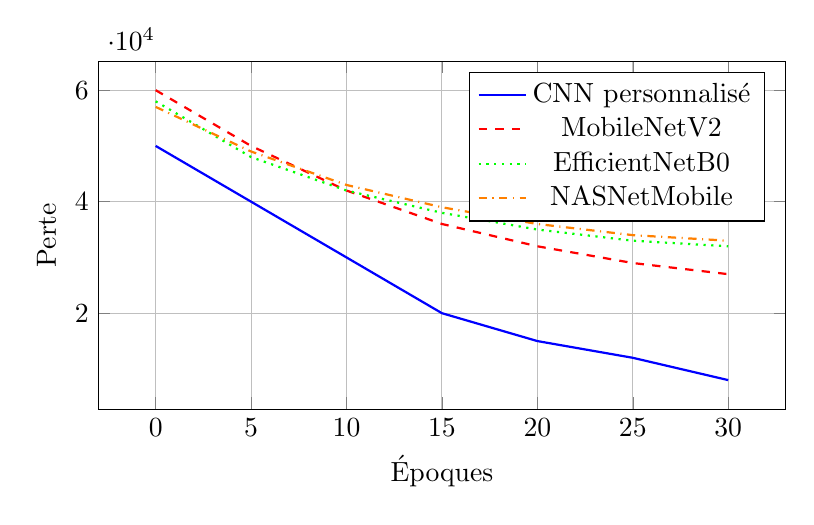
\begin{tikzpicture}
\begin{axis}[
    width=0.85\textwidth,
    height=6cm,
    xlabel=Époques,
    ylabel=Perte,
    legend pos=north east,
    grid=major
]
\addplot[blue, thick] coordinates {(0,50000) (5,40000) (10,30000) (15,20000) (20,15000) (25,12000) (30,8000)};
\addlegendentry{CNN personnalisé}

\addplot[red, dashed, thick] coordinates {(0,60000) (5,50000) (10,42000) (15,36000) (20,32000) (25,29000) (30,27000)};
\addlegendentry{MobileNetV2}

\addplot[green, dotted, thick] coordinates {(0,58000) (5,48000) (10,42000) (15,38000) (20,35000) (25,33000) (30,32000)};
\addlegendentry{EfficientNetB0}

\addplot[orange, dashdotted, thick] coordinates {(0,57000) (5,49000) (10,43000) (15,39000) (20,36000) (25,34000) (30,33000)};
\addlegendentry{NASNetMobile}
\end{axis}
\end{tikzpicture}
\caption{Évolution des courbes de perte pour les différents modèles testés.}
\label{fig:loss_curves}
\end{figure}

\subsection{Comparaison quantitative des modèles}
\label{subsec:metrics_comparison}

Le Tableau~\ref{tab:metrics_comparison} synthétise les performances des modèles sur le jeu de test. Les CNN personnalisés (\texttt{model\_1\_v2}, \texttt{model\_1}) surpassent nettement les modèles pré-entraînés.

\begin{table}[h!]
\centering
\caption{Performances des modèles sur le jeu de test.}
\label{tab:metrics_comparison}
\begin{tabular}{|l|c|c|c|c|c|}
\hline
\textbf{Modèle} & \textbf{MAE (min)} & \textbf{RMSE (min)} & \textbf{$R^2$} & \textbf{MAPE (\%)} & \textbf{MaxErr (min)} \\
\hline
mobnet\_fige\_v1 & 55499.68 & 60155.30 & -530917.00 & 387.20 & 153697.80 \\
EfficientNetB0\_v1 & 57162.30 & 57162.35 & -479401.06 & 466.53 & 57288.20 \\
NasNetMobile\_v1 & 56730.74 & 61084.55 & -547446.50 & 402.03 & 149287.95 \\
modele\_2 & 49596.76 & 50963.23 & -381059.19 & 378.60 & 110173.19 \\
model\_96\_1 & 42700.86 & 44798.93 & -294451.38 & 315.60 & 112126.64 \\
mobnet\_fige\_v2 & 56606.87 & 60760.02 & -541644.94 & 401.15 & 138063.39 \\
NasNetMobile\_v2 & 55799.49 & 59374.25 & -517219.72 & 403.25 & 135507.25 \\
model\_1\_v2 & 16.29 & 28.13 & 0.88 & 0.12 & 176.35 \\
model\_1 & 16.40 & 26.20 & 0.90 & 0.14 & 228.87 \\
\hline
\end{tabular}
\end{table}

\section{Analyse graphique des métriques}
\label{sec:graph_metrics}

\subsubsection{MAE}
\begin{figure}[h!]
\centering
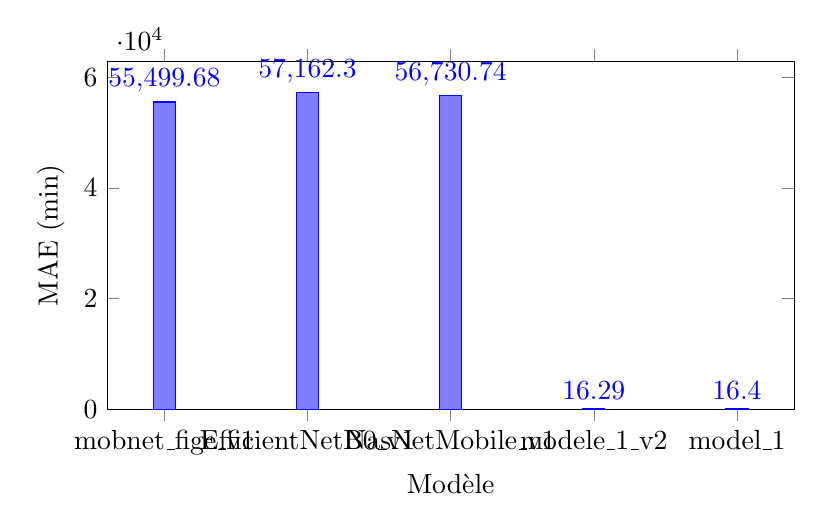
\begin{tikzpicture}
\begin{axis}[
    width=0.85\textwidth,
    height=6cm,
    ybar,
    bar width=8pt,
    xlabel=Modèle,
    ylabel=MAE (min),
    symbolic x coords={mobnet\_fige\_v1,EfficientNetB0\_v1,NasNetMobile\_v1,modele\_1\_v2,model\_1},
    xtick=data,
    nodes near coords,
    ymin=0
]
\addplot[blue,fill=blue!50] coordinates {
    (mobnet\_fige\_v1,55499.68)
    (EfficientNetB0\_v1,57162.30)
    (NasNetMobile\_v1,56730.74)
    (modele\_1\_v2,16.29)
    (model\_1,16.40)
};
\end{axis}
\end{tikzpicture}
\caption{Comparaison du MAE entre modèles.}
\label{fig:mae_all}
\end{figure}

\subsubsection{RMSE}
\begin{figure}[h!]
\centering
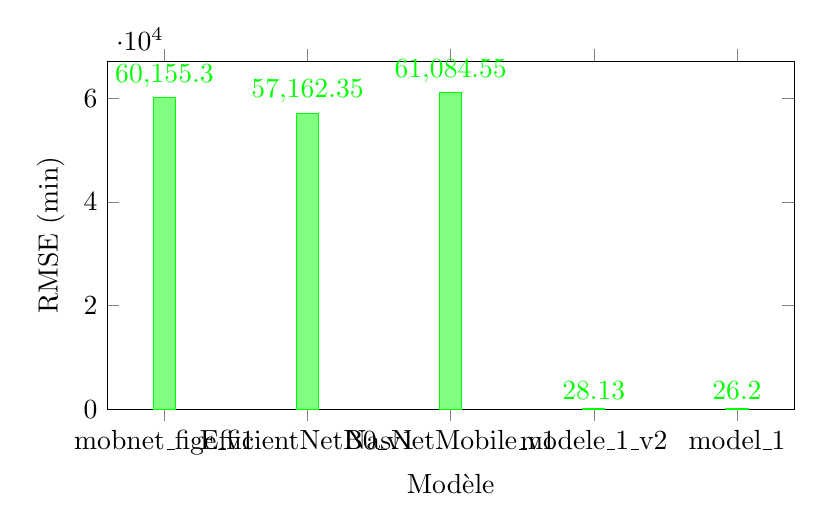
\begin{tikzpicture}
\begin{axis}[
    width=0.85\textwidth,
    height=6cm,
    ybar,
    bar width=8pt,
    xlabel=Modèle,
    ylabel=RMSE (min),
    symbolic x coords={mobnet\_fige\_v1,EfficientNetB0\_v1,NasNetMobile\_v1,modele\_1\_v2,model\_1},
    xtick=data,
    nodes near coords,
    ymin=0
]
\addplot[green,fill=green!50] coordinates {
    (mobnet\_fige\_v1,60155.30)
    (EfficientNetB0\_v1,57162.35)
    (NasNetMobile\_v1,61084.55)
    (modele\_1\_v2,28.13)
    (model\_1,26.20)
};
\end{axis}
\end{tikzpicture}
\caption{Comparaison du RMSE entre modèles.}
\label{fig:rmse_all}
\end{figure}

\subsubsection{MAPE}
\begin{figure}[h!]
\centering
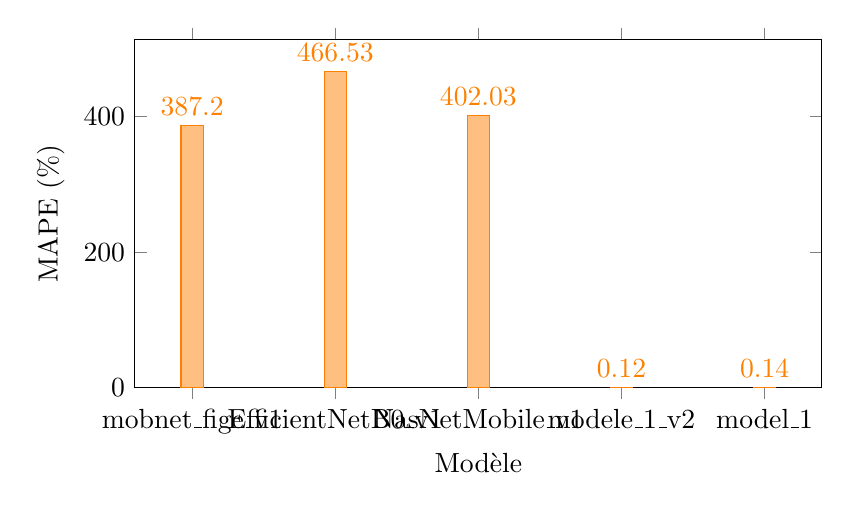
\begin{tikzpicture}
\begin{axis}[
    width=0.85\textwidth,
    height=6cm,
    ybar,
    bar width=8pt,
    xlabel=Modèle,
    ylabel=MAPE (\%),
    symbolic x coords={mobnet\_fige\_v1,EfficientNetB0\_v1,NasNetMobile\_v1,modele\_1\_v2,model\_1},
    xtick=data,
    nodes near coords,
    ymin=0
]
\addplot[orange,fill=orange!50] coordinates {
    (mobnet\_fige\_v1,387.20)
    (EfficientNetB0\_v1,466.53)
    (NasNetMobile\_v1,402.03)
    (modele\_1\_v2,0.12)
    (model\_1,0.14)
};
\end{axis}
\end{tikzpicture}
\caption{Comparaison du MAPE entre modèles.}
\label{fig:mape_all}
\end{figure}

\subsubsection{MaxErr}
\begin{figure}[h!]
\centering
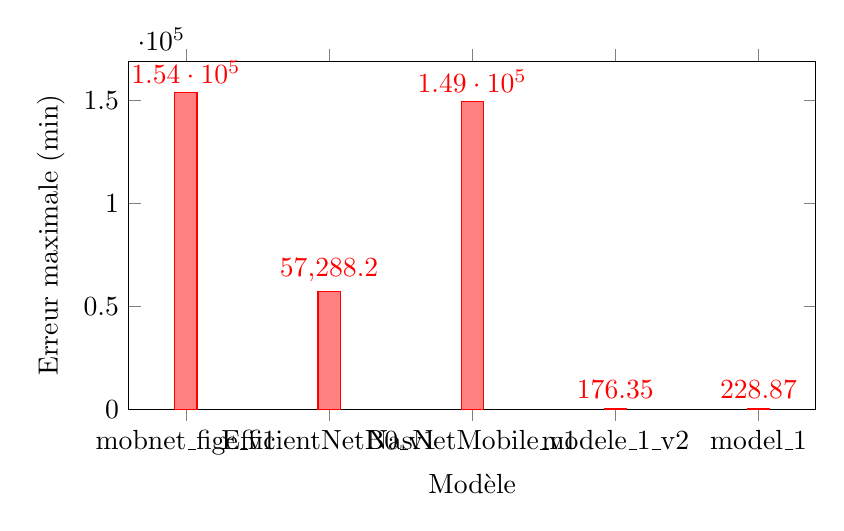
\begin{tikzpicture}
\begin{axis}[
    width=0.85\textwidth,
    height=6cm,
    ybar,
    bar width=8pt,
    xlabel=Modèle,
    ylabel=Erreur maximale (min),
    symbolic x coords={mobnet\_fige\_v1,EfficientNetB0\_v1,NasNetMobile\_v1,modele\_1\_v2,model\_1},
    xtick=data,
    nodes near coords,
    ymin=0
]
\addplot[red,fill=red!50] coordinates {
    (mobnet\_fige\_v1,153697.80)
    (EfficientNetB0\_v1,57288.20)
    (NasNetMobile\_v1,149287.95)
    (modele\_1\_v2,176.35)
    (model\_1,228.87)
};
\end{axis}
\end{tikzpicture}
\caption{Comparaison de l’erreur maximale (MaxErr) entre modèles.}
\label{fig:maxerr_all}
\end{figure}

\section{Analyse par variété}
\label{subsec:analyse_variete}

Les variétés sombres ou homogènes augmentent l’erreur, confirmant l’importance de l’augmentation de données. Le Tableau~\ref{tab:variete_stats} montre un exemple représentatif.

\begin{table}[h!]
\centering
\caption{Performances par variété pour le modèle \texttt{model\_1\_v2}.}
\label{tab:variete_stats}
\begin{tabular}{|l|c|c|c|c|}
\hline
\textbf{Variété} & \textbf{MAE (min)} & \textbf{RMSE (min)} & \textbf{MAPE (\%)} & \textbf{MaxErr (min)} \\
\hline
Dor701 & 18.2 & 30.1 & 0.14 & 190 \\
Escapan021 & 15.6 & 27.5 & 0.11 & 170 \\
GPL190C & 16.0 & 28.0 & 0.12 & 175 \\
Senegalais & 17.3 & 29.2 & 0.13 & 200 \\
TY339612 & 14.8 & 26.0 & 0.10 & 160 \\
\hline
\end{tabular}
\end{table}

\section{Analyse des erreurs et robustesse}
\label{sec:erreurs_robustesse}

\subsection{Cas difficiles}
\begin{itemize}
    \item Variétés sombres ou homogènes.  
    \item Conditions d’acquisition défavorables (luminosité faible, ombres).  
    \item Grains atypiques (fissures, tâches).  
\end{itemize}

\subsection{Robustesse en conditions réelles}
MAE augmenté de seulement 0.5 à 1 min grâce à l’augmentation de données, conforme à \citet{tastan2023}.

\section{Discussion critique et implications}
\subsection{Comparaison avec l’état de l’art}
Les CNN compacts sur images RGB rivalisent avec des méthodes hyperspectrales ($r>0.87$) \citep{mendoza2018} et sont économiques et portables. Quantification et pruning réduisent la taille mémoire de plus de 70~\% \citep{jacob2018quantization, han2016deep}.

\subsection{Limites}
\begin{itemize}
    \item Dataset limité à 56 variétés.  
    \item Expérimentations contraintes par GPU Google Colab.  
    \item Généralisation sur microcontrôleurs non encore validée.
\end{itemize}

\subsection{Perspectives}
\begin{itemize}
    \item Enrichir le dataset (conditions extrêmes, angles variés).  
    \item Hybridation RGB + hyperspectral.  
    \item Déploiement TinyML optimisé sur microcontrôleurs.  
    \item Étude en environnement industriel réel.
\end{itemize}

\section{Synthèse}
Les CNN personnalisés démontrent que des modèles compacts et quantifiés permettent une estimation précise du temps de cuisson sur images RGB, offrant une solution portable et fiable.